\section{Introduction}\label{sec:intro}
Microservice systems are increasingly appealing to cloud-native enterprise applications for several reasons, including resource flexibility, loosely-coupled architecture, and lightweight deployment~\cite{Ali21Survey}.
However, anomalies are inevitable in microservices due to their complexity and dynamism. An anomaly in one microservice could propagate to others and magnify its impact, resulting in considerable revenue and reputation loss for companies~\cite{IndSurvey21Zhou}.
Figure~\ref{fig:dependency-graph} shows an example where a failure in one microservice may delay all microservices on the invocation chain.
\begin{figure}[htb]
    \centering
        {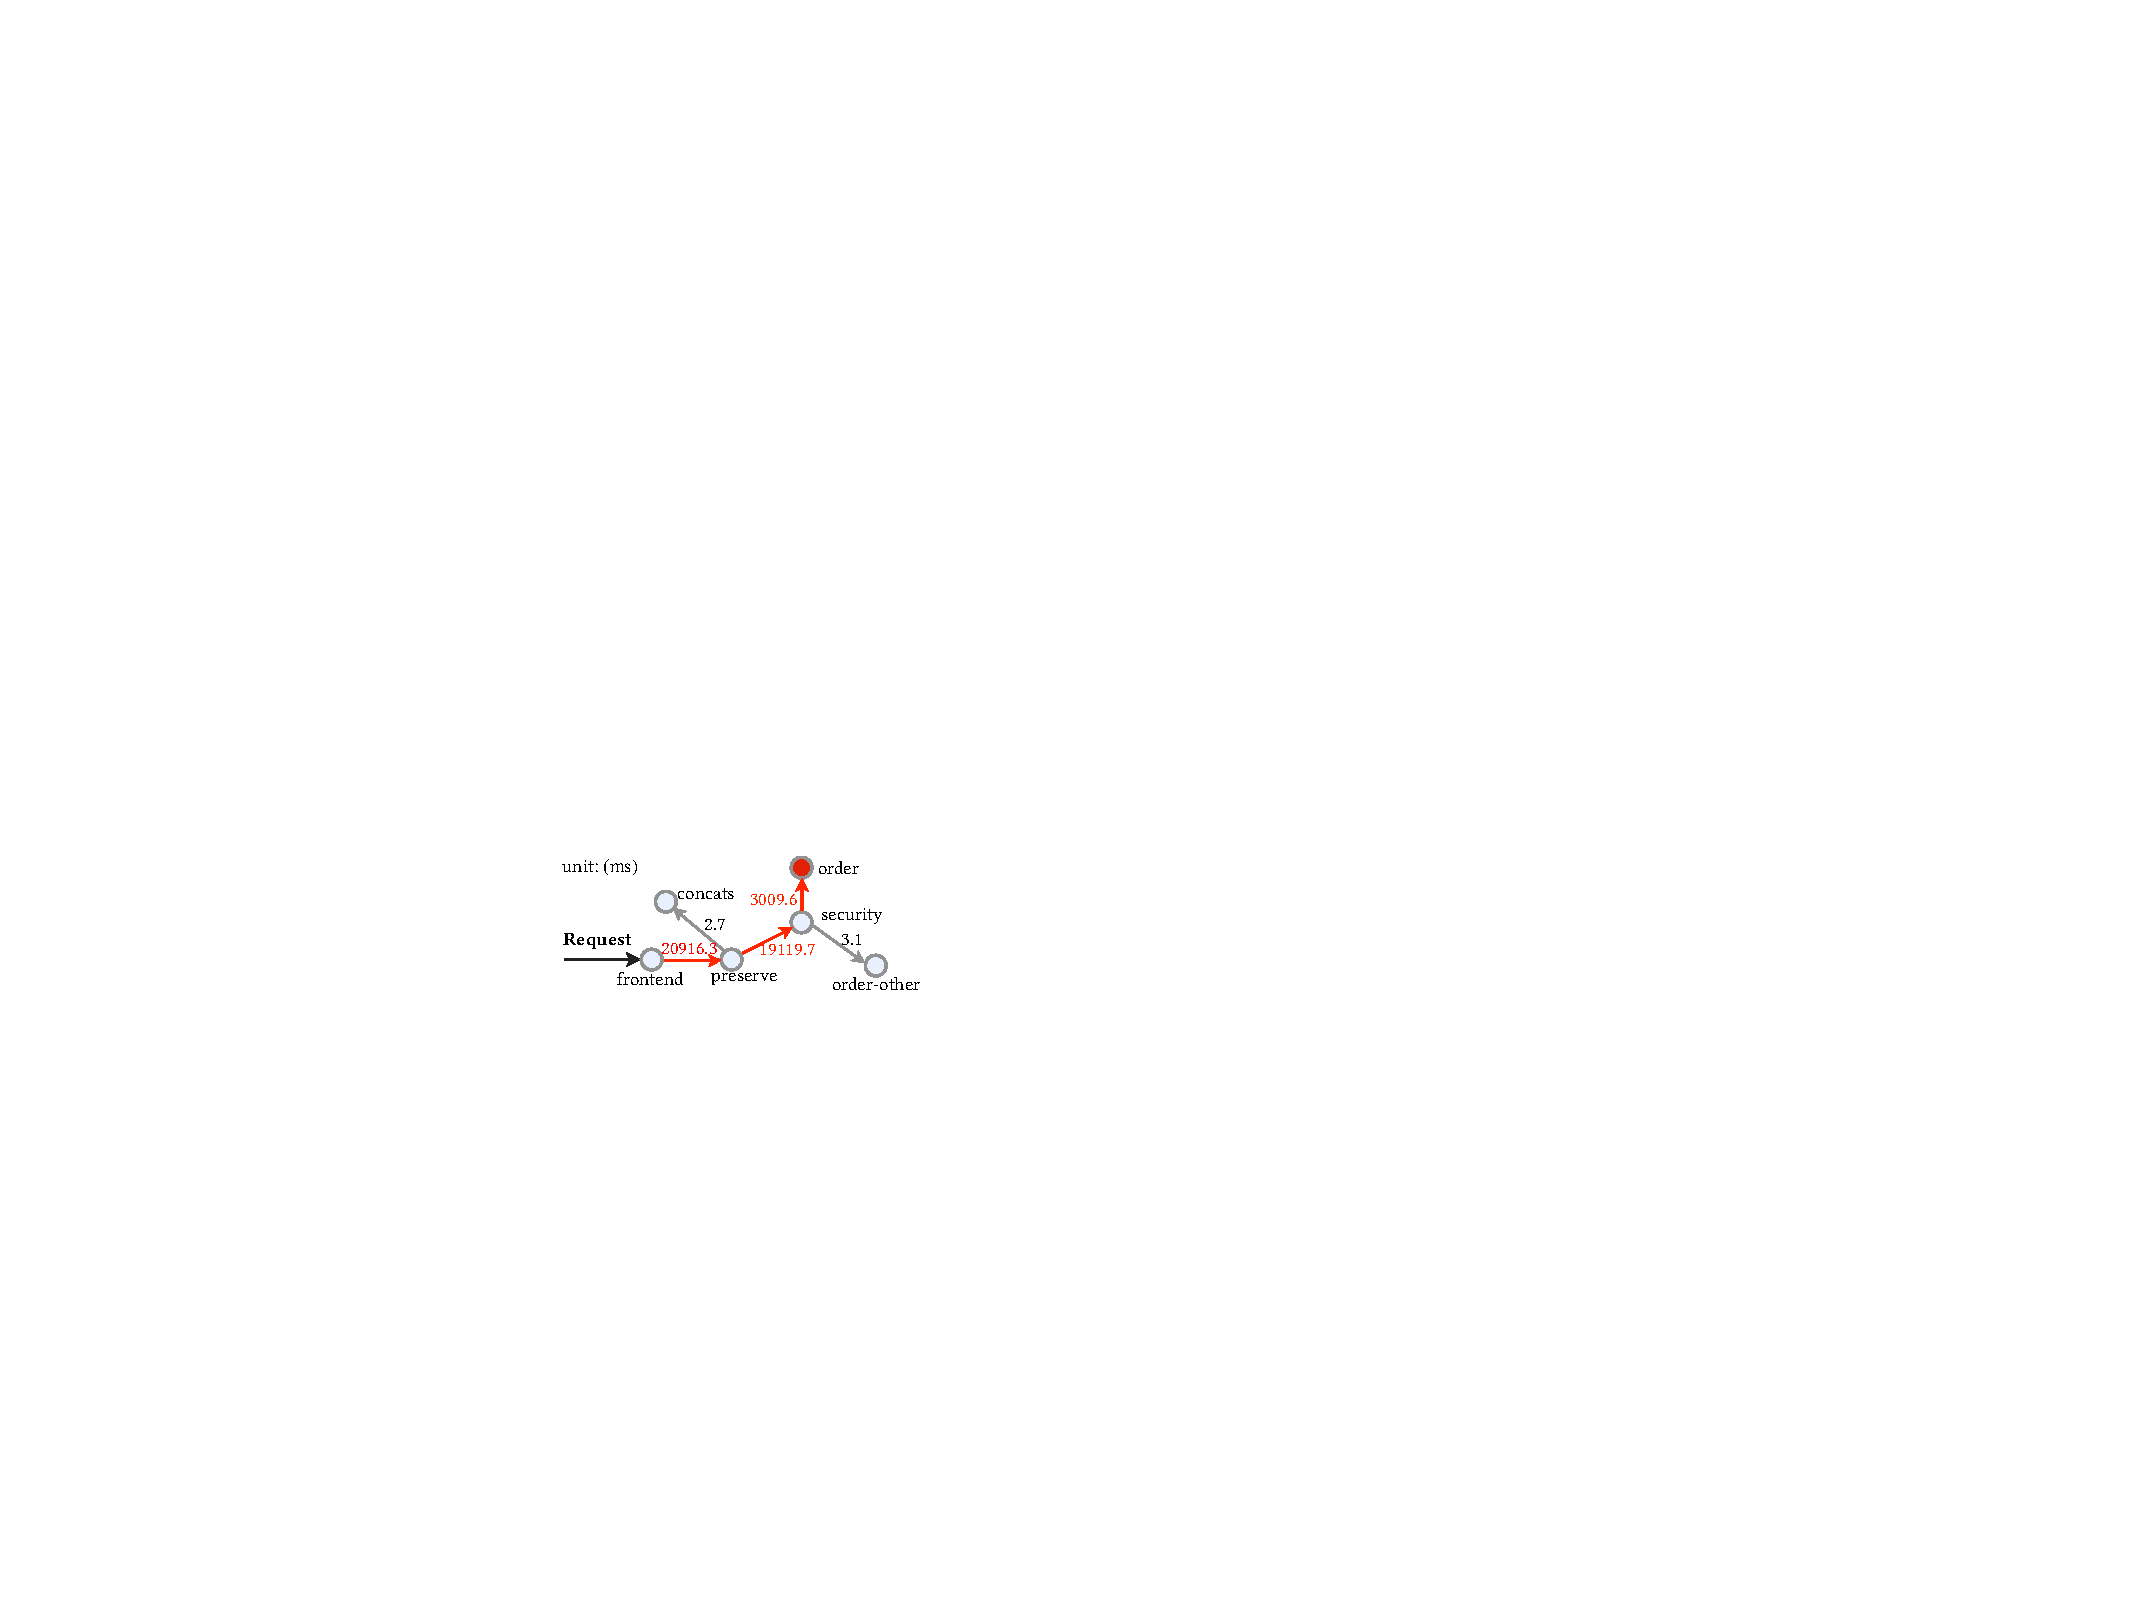
\includegraphics[width=0.65\linewidth]{figures/dependency.pdf}}
    \caption{A failure in ``order'' indirectly delays other microservices on the invocation chain, while microservices off the chain are unaffected.}
    \label{fig:dependency-graph}
\end{figure}

Therefore, developers must closely monitor the microservice status via run-time information (e.g., traces, system logs, and KPIs) to discover and tackle potential failures in their earliest efforts.
Yet, thousands of microservices are usually running in distributed machines in a large-scale industrial microservice system. As each microservice can launch multiple instances, a system can produce billions of run-time records per day~\cite{IndSurvey21Zhou, Ali21Survey}. The explosion of monitoring data makes automated troubleshooting techniques imperative.

Many efforts have been devoted to this end, focusing either on anomaly detection~\cite{TraceAnomaly, MMTrace, DeepTraLog} or on root cause localization~\cite{DyCause, MicroCause, MonitorRank, MicroHECL, TBAC, CloudRanger}. Anomaly detection tells whether an anomaly exists, and root cause localization identifies the culprit microservice upon the existence of an anomaly.
Previous approaches usually leverage statistical models or machine learning techniques to mine information from traces, as traces profile and monitor microservice executions and record essential inter-service information (e.g., request duration).
However, we identify two main limitations of the existing troubleshooting approaches.

(1) \textit{Insufficient exploitation of monitoring data}:
different from operation teams that pay close attention to diverse sources of run-time information, existing research deeply relies on traces and exploits other data sources insufficiently. 
This gap stems from the complexity of multi-source data analysis, which is much harder than single-source data analysis, as multi-source data is heterogeneous, frequently interacting, and very large~\cite{Multisource}.
However, on the one hand, traces contain important information for troubleshooting but are insufficient to reveal all typical types of anomalies.
On the other hand, different types of data, such as logs and KPIs, can reveal anomalies collaboratively and bring more clues about potential failures.
For example, a CPU exhaustion fault can cause abnormally high values in the CPU usage indicator and trigger warnings recorded in logs, but the traces may not exhibit abnormal patterns (such as high latency).

(2) \textit{Disconnection in closely related tasks}:
Generally, root cause localization follows anomaly detection since we must discover an anomaly before analyzing it.
Current studies of microservice reliability regard the two phases as independent, despite their shared inputs and knowledge about the microservice status. Existing approaches usually deal with the same inputs redundantly and waste the rich correlation information between anomaly detection and root cause localization.
Moreover, the contradiction between computing efficiency and accuracy limits the simple combination of state-of-the-art anomaly detectors and root cause localizers.
For a two-stage troubleshooting approach, it is generally a little late to use an advanced anomaly detector and then analyze the root cause.
Thus, root cause localization-focused studies usually apply oversimplified anomaly detectors (e.g., N-sigma), and unfortunately, the resulting detection outputs can contain many noisy labels and thereby affect the effectiveness of downstream root cause localization. 

To overcome the above limitations, we propose \textbf{\name}, the first \underline{E}nd-to-end framework integrating \underline{A}nomaly \underline{D}etection and \underline{R}oot cause l\underline{O}calization to troubleshoot microservice systems based on multi-source monitoring data.
The key ideas are 1) learning discriminative representations of the microservice status via multi-modal learning and 2) forcing the model to learn fundamental features revealing anomalies via multi-task learning.
Therefore, \name can fully exploit meaningful information from different data sources that can all manifest anomalies. Also, it allows information to be inputted once and used to tackle anomaly detection and root cause localization together and avoids incorrect detection results hindering next-phase root cause localization.

Specifically, \name consists of three components:
\textit{(1) Modal-wise learning} contains modality-specific modules for learning intra-service behaviors from logs, KPIs, and traces. 
We apply Hawkes process~\cite{Hawkes} and a fully connected (FC) layer to model the log event occurrences.
KPIs are fed into a dilated causal convolution (DCC) layer~\cite{TCN} to learn temporal dependencies and inter-series associations.
We also use DCC to capture meaningful fluctuations of latency in traces, such as extremely high values.
\textit{(2) Dependency-aware status learning} aims to model the intra- and inter-dependencies between microservices.
It first fuses the multi-modal representations via gated concentration and feeds the fused representation into a graph attention network (GAT), where the topological dependency is built on historical invocations.
\textit{(3) Joint detection and localization} contains an anomaly detector and a root cause localizer sharing representations and an objective. It predicts the existence of anomalies and the probability of each microservice being the culprit upon an anomaly alarm.

Experimental results on two datasets collected from two widely-used benchmark microservice systems demonstrate the effectiveness of \name. 
For anomaly detection, \name surpasses all compared approaches by a large margin 
in \textit{F1} (53.82\%\textasciitilde92.68\%), and also increases \textit{F1} by 11.47\% on average compared to our derived multi-source data-based methods.
For root cause localization, \name achieves state-of-the-art results with 290\%\textasciitilde5068\% higher in \textit{HR@1} (Top-1 Hit Rate) than five advanced baselines and outperforms our derived methods by 43.06\% in \textit{HR@1} on average.
An extensive ablation study further confirms the contributions of modeling different data sources.

Our main contributions are highlighted as follows:
\begin{itemize}%[leftmargin=10pt, topsep=0pt]
\setlength\itemsep{0em}
   
   \item We identify two limitations of existing approaches for troubleshooting microservices, motivated by which we are the first to explore the opportunity and necessity to integrate anomaly detection and root cause localization, as well as exploit logs, KPIs, and traces together.
    
    \item We propose the first end-to-end troubleshooting framework (\name) to jointly conduct anomaly detection and root cause localization for microservices based on multi-source data. \name models intra-service behaviors and inter-service dependencies.
    
    \item We conduct extensive experiments on two benchmark datasets. The results demonstrate that \name outperforms all compared approaches, including state-of-the-art approaches and derived multi-source baselines on both anomaly detection and root cause localization. We also conduct ablation studies to further validate the contributions of different data sources. 
    
    \item Our code and data~\footnote{https://github.com/BEbillionaireUSD/Eadro} are made public for practitioners to adopt, replicate or extend \name.
    
\end{itemize}
